%!Tex Root = ../main.tex
% ./Packete.tex
% ./Design.tex
% ./Deklarationen.tex
% ./Vorbereitung.tex
% ./Aufgabe1.tex
% ./Aufgabe2.tex
% ./Aufgabe3.tex
% ./Appendix.tex

\section{Aufgabe 4}

\setcounter{exercise}{1}

\begin{frame}{Aufgabe \thesection}{D-Flip-Flop}
  \begin{solutionnoinc}
    \begin{columns}
      \begin{column}{0.5\textwidth}
        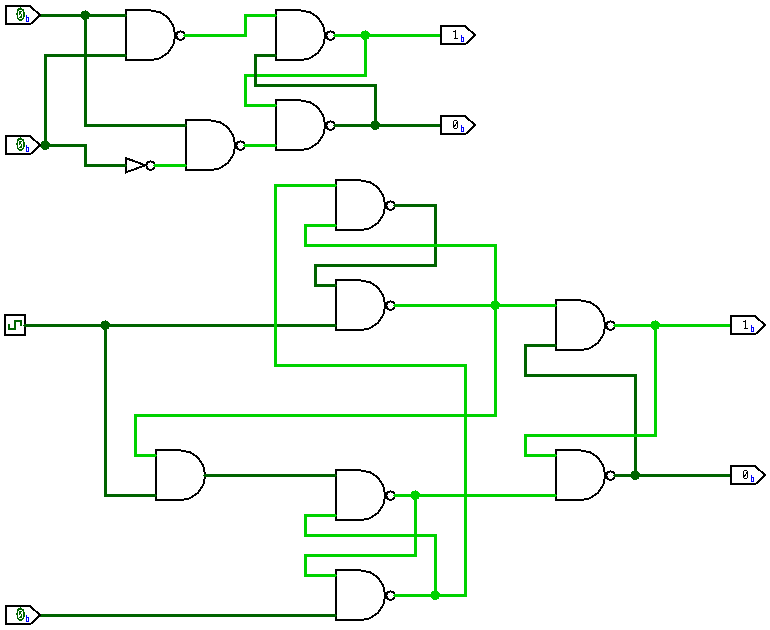
\includegraphics[height=0.5\paperheight, center]{./figures/comparison001.png}
      \end{column}
      \begin{column}{0.5\textwidth}
        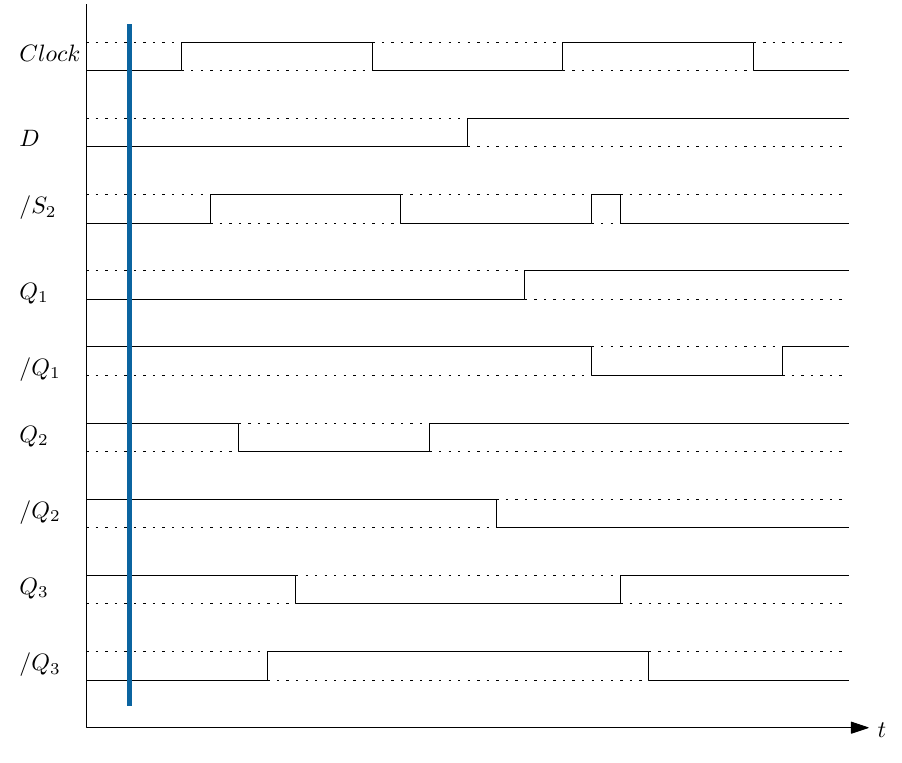
\includegraphics[height=0.5\paperheight, center]{./figures/timing_diagram_1.png}
      \end{column}
    \end{columns}
  \end{solutionnoinc}
\end{frame}
\begin{frame}{Aufgabe \thesection}{D-Flip-Flop}
  \begin{solutionnoinc}
    \begin{columns}
      \begin{column}{0.5\textwidth}
        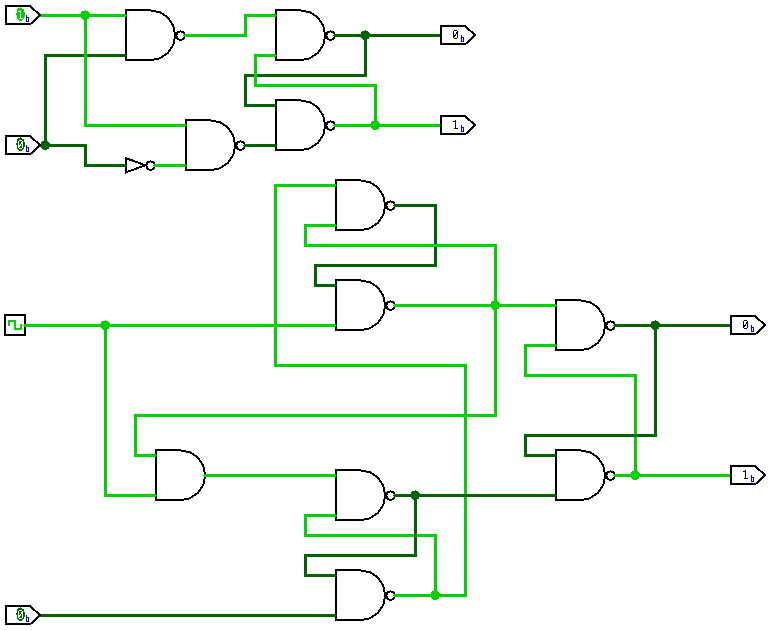
\includegraphics[height=0.5\paperheight, center]{./figures/comparison100.png}
      \end{column}
      \begin{column}{0.5\textwidth}
        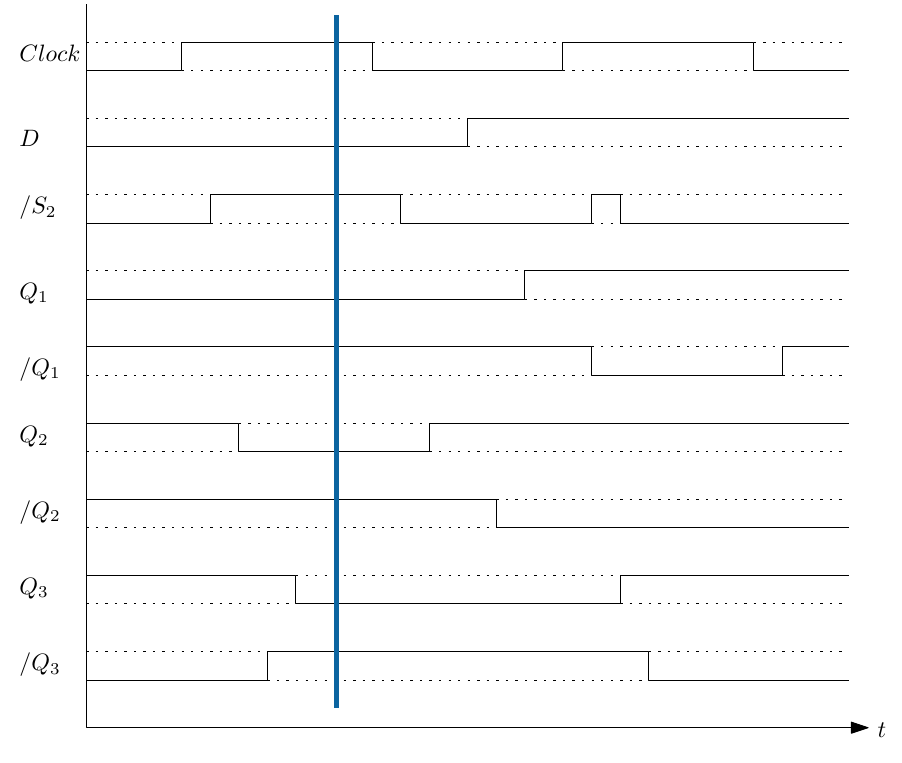
\includegraphics[height=0.5\paperheight, center]{./figures/timing_diagram_2.png}
      \end{column}
    \end{columns}
  \end{solutionnoinc}
\end{frame}
\begin{frame}{Aufgabe \thesection}{D-Flip-Flop}
  \begin{solutionnoinc}
    \begin{columns}
      \begin{column}{0.5\textwidth}
        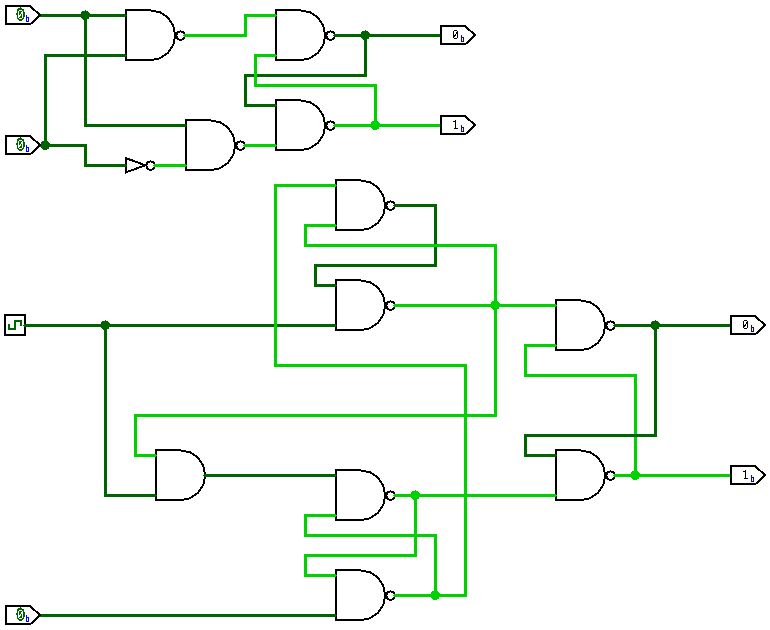
\includegraphics[height=0.5\paperheight, center]{./figures/comparison000.png}
      \end{column}
      \begin{column}{0.5\textwidth}
        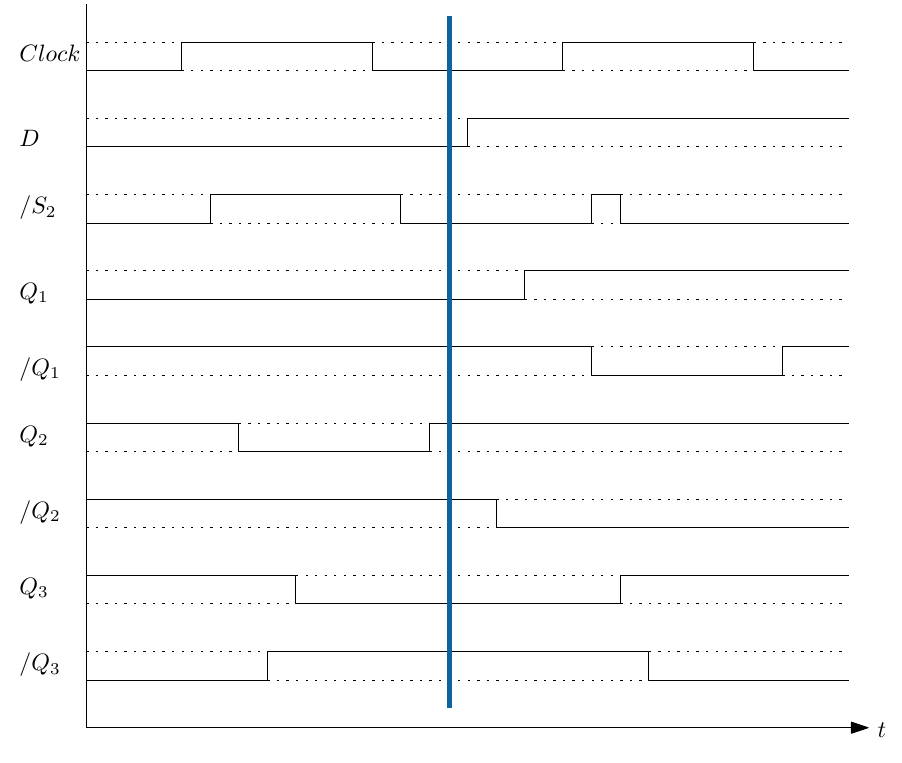
\includegraphics[height=0.5\paperheight, center]{./figures/timing_diagram_3.png}
      \end{column}
    \end{columns}
  \end{solutionnoinc}
\end{frame}
\begin{frame}{Aufgabe \thesection}{D-Flip-Flop}
  \begin{solutionnoinc}
    \begin{columns}
      \begin{column}{0.5\textwidth}
        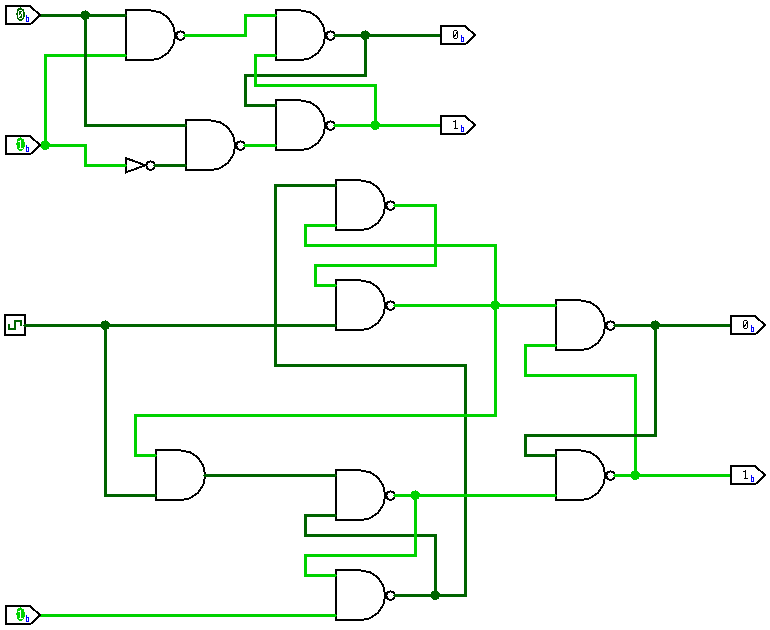
\includegraphics[height=0.5\paperheight, center]{./figures/comparison010.png}
      \end{column}
      \begin{column}{0.5\textwidth}
        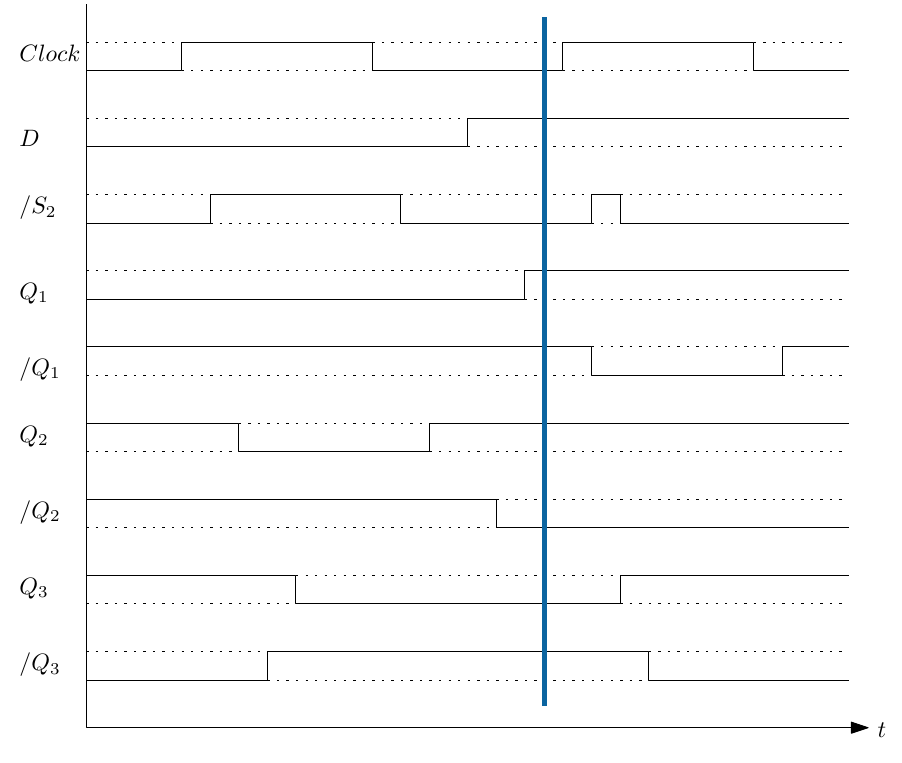
\includegraphics[height=0.5\paperheight, center]{./figures/timing_diagram_4.png}
      \end{column}
    \end{columns}
  \end{solutionnoinc}
\end{frame}
\begin{frame}{Aufgabe \thesection}{D-Flip-Flop}
  \begin{solutionnoinc}
    \begin{columns}
      \begin{column}{0.5\textwidth}
        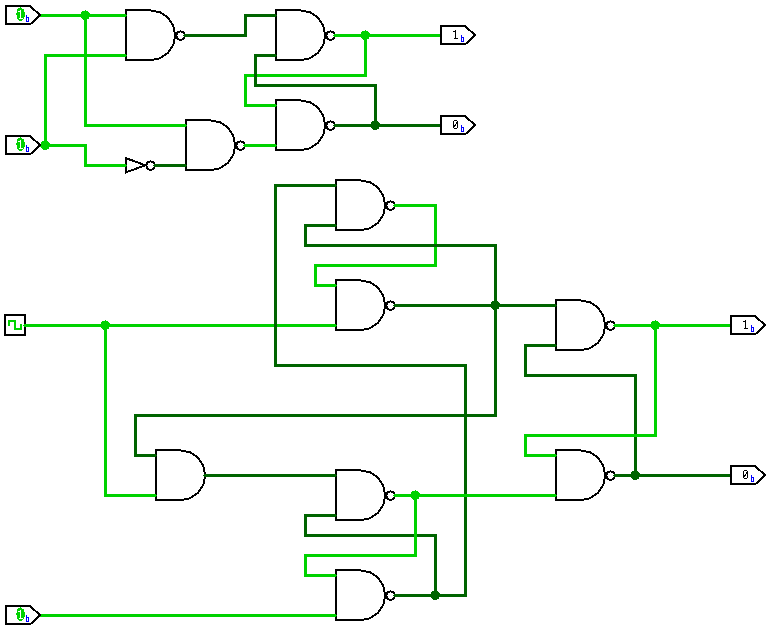
\includegraphics[height=0.5\paperheight, center]{./figures/comparison111.png}
      \end{column}
      \begin{column}{0.5\textwidth}
        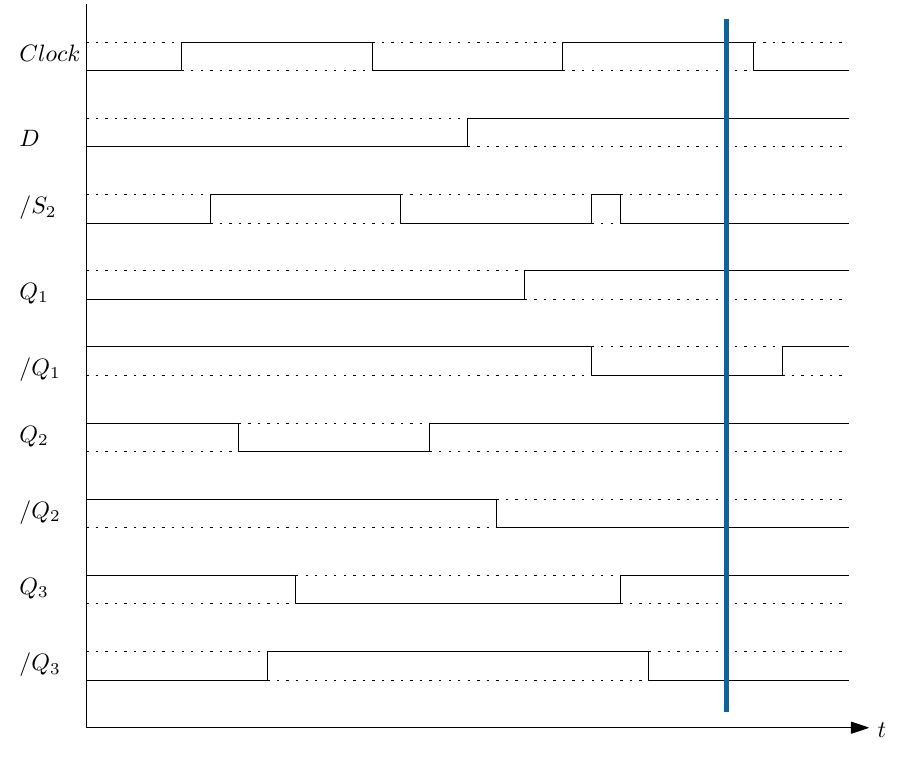
\includegraphics[height=0.5\paperheight, center]{./figures/timing_diagram_5.png}
      \end{column}
    \end{columns}
  \end{solutionnoinc}
\end{frame}
\begin{frame}{Aufgabe \thesection}{D-Flip-Flop}
  \begin{solutionnoinc}
    \begin{columns}
      \begin{column}{0.5\textwidth}
        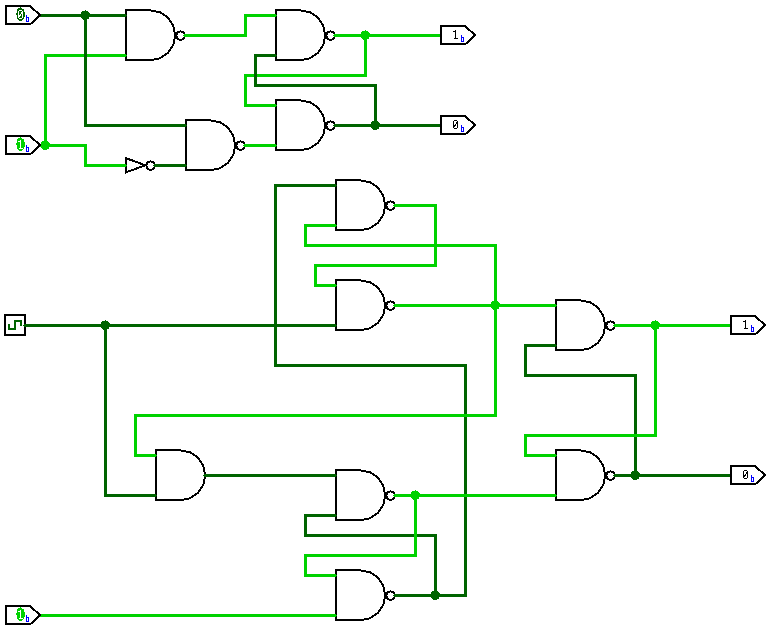
\includegraphics[height=0.5\paperheight, center]{./figures/comparison011.png}
      \end{column}
      \begin{column}{0.5\textwidth}
        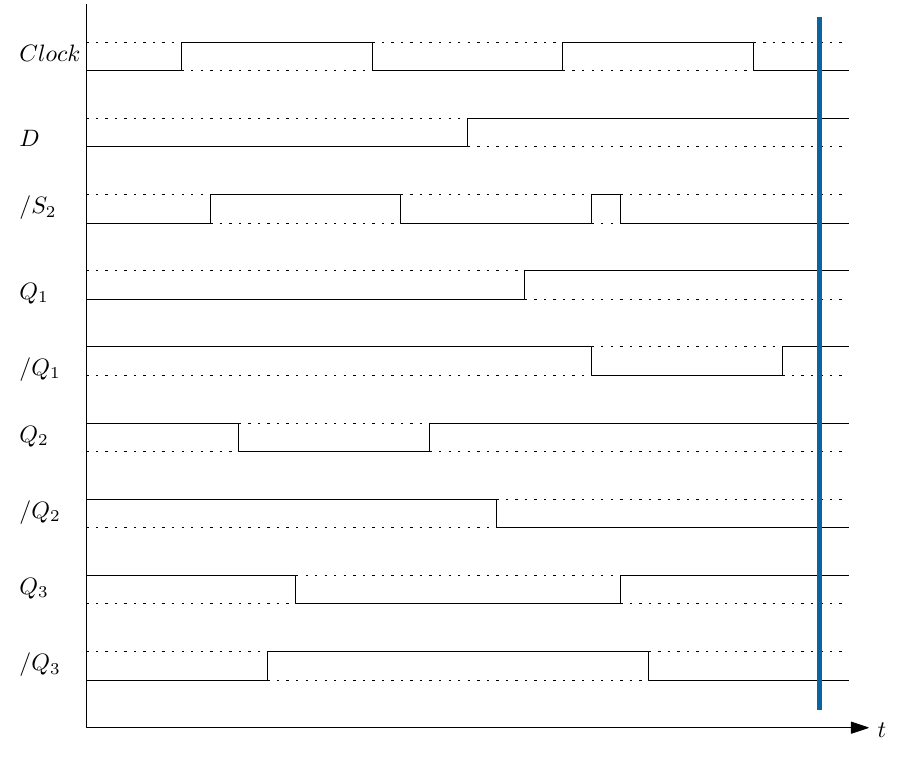
\includegraphics[height=0.5\paperheight, center]{./figures/timing_diagram_6.png}
      \end{column}
    \end{columns}
  \end{solutionnoinc}
\end{frame}
